\section{Nota teórica}
\subsection{Información general del MCU}

El microcontrolador ($\mu C$) utilizado en este laboratorio es el PIC12F675 del fabricante \textit{Microchip}, el cual se trata de un microcontrolador de 8 bits tipo CMOS. 
Consta de una célda FLASH de 1024 palabras para alamacenar la memoria de programa. Posee 4 canales de conversión analógico a digital (ADC), 1 canal de comparador, resistores \textit{pull-up} programables, 4 selecciones de osciladores, y 128 bytes de memoria EEPROM.
El diagrama de pines del $\mu C$ se muestra a contiuación:

\begin{figure}[!h]
    \centering
    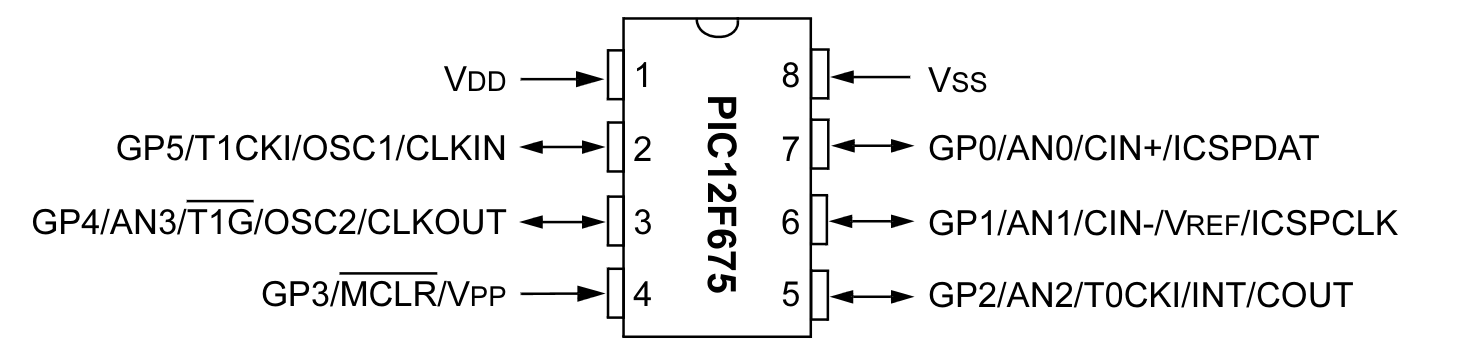
\includegraphics[width = 0.8\linewidth]{imagenes/fig1.png}
    \caption{Diagrama de pines del $\mu C$ PIC12F675}
    \label{fig1}
\end{figure}

Además, este microcontrolador posee una arquitectura RISC de alto rendimiento, la cual consiste de 35 instrucciones y una frecuencia de operación de \SI{20}{MHz}. 
Este microcontrolador es fácilmente adaptable para aplicaciones automotrices, industriales, y para aplicaciones de menor escala gracias a su reprogramibilidad. 
Sus características eléctricas se resumen en la siguiente tabla:

\begin{figure}[!h]
    \centering
    \begin{tabular}{lr}
          \toprule
          Característica eléctrica& Valor máximo absoluto\\ 
          \midrule
          Temperatura ambiente mientras esté polarizado & \SI{-40}{\degreeCelsius} a \SI{+125}{\degreeCelsius}\\
          Temperatura de almacenamiento & \SI{-65}{\degreeCelsius} a \SI{+150}{\degreeCelsius}\\
          Voltaje en $V_{DD}$ con respecto a $V_{SS}$ & \SI{-0.3}{V} a \SI{+6.5}{V}\\
          Voltaje en $\overline{MCLR}$ con respecto a $V_{SS}$ & \SI{-0.3}{V} a \SI{+13.5}{V}\\
          Voltaje en todos los otros pines con respecto a $V _{SS}$ & \SI{-0.3}{V} a $(V _{DD} + \SI{0.3}{V})$\\
          Potencia total disipada & \SI{800}{mW}\\
          Corriente máxima saliente en el pin $V _{SS}$ & \SI{300}{mA}\\
          Corriente máxima entrante en el pin $V _{DD}$ & \SI{250}{mA}\\
          Corriente clamp de entrada $I _{IK}$ $(V _{I}<0\ \text{o}\ V _{I}>V _{DD})$ & $\pm \SI{20}{mA}$\\
          Corriente clamp de salida $I _{OK}$ $(V _{O}<0\ \text{o}\ V _{O}>V _{DD})$ & $\pm \SI{20}{mA}$\\
          Corriente máxima de salida sourced por cualquier pin I/O & \SI{25}{mA}\\
          Corriente máxima de salida sinked por cualquier pin I/O & \SI{25}{mA}\\
          Corriente máxima sunked por todos los pines GPIO & \SI{125}{mA}\\
          Corriente máxima sourced por todos los pines GPIO & \SI{125}{mA}\\
          \bottomrule
      \end{tabular}
    \caption{Especificaciones eléctricas del $\mu C$ PIC12F675}
    \label{t1}
\end{figure}

Con respecto a los periféricos con los cuales cuenta el PIC12F675, posee 6 pines I/O, un módulo de conversión analógico a digital con una resolución de 10 bits con canales programables, un módulo de comparador analógico programable, 2 timers, Timer0 de 8 bits y Timer1 de 16 bits con prescaler programables, y por último, posee la habilidad de ser programado después de que el $\mu C$ haya sido instalado dentro de un sistema completo (ICSP™, In-Circuit Serial Programming™).

El diagrama de bloques de la estructura interna del PIC12F675 se muestra a continuación:
\vfill
\begin{figure}[!h]
    \centering
    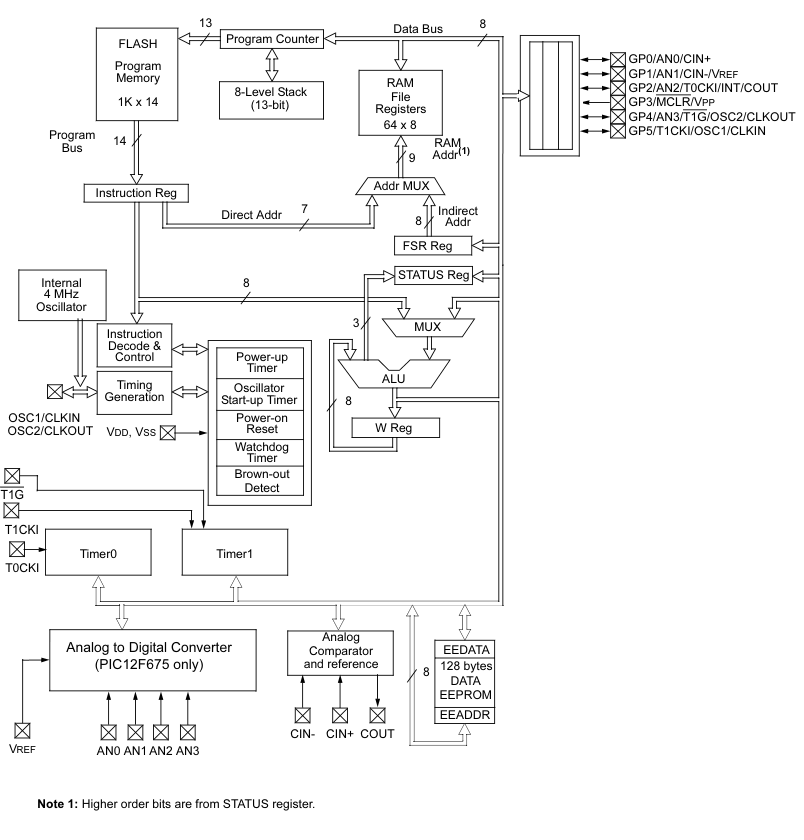
\includegraphics[width = \linewidth]{imagenes/fig2.png}
    \caption{Diagrama de bloques del $\mu C$ PIC12F675}
    \label{fig2}
\end{figure}
\vfill
\newpage
\subsection{Periféricos}


